%% NSS-MIC_Instructions.tex
%% 8/2007
%% By Bo Yu (yu@bnl.gov)
%% based on:
%% bare_jrnl.tex
%% V1.3
%% 2007/01/11
%% by Michael Shell
%% see http://www.michaelshell.org/
%% for current contact information.
%%
%% This is a skeleton file demonstrating the use of IEEEtran.cls
%% (requires IEEEtran.cls version 1.7 or later) with an IEEE journal paper.
%%
%% Support sites:
%% http://www.michaelshell.org/tex/ieeetran/
%% http://www.ctan.org/tex-archive/macros/latex/contrib/IEEEtran/
%% and
%% http://www.ieee.org/

%%*************************************************************************
%% Legal Notice:
%% This code is offered as-is without any warranty either expressed or
%% implied; without even the implied warranty of MERCHANTABILITY or
%% FITNESS FOR A PARTICULAR PURPOSE! 
%% User assumes all risk.
%% In no event shall IEEE or any contributor to this code be liable for
%% any damages or losses, including, but not limited to, incidental,
%% consequential, or any other damages, resulting from the use or misuse
%% of any information contained here.
%%
%% All comments are the opinions of their respective authors and are not
%% necessarily endorsed by the IEEE.
%%
%% This work is distributed under the LaTeX Project Public License (LPPL)
%% ( http://www.latex-project.org/ ) version 1.3, and may be freely used,
%% distributed and modified. A copy of the LPPL, version 1.3, is included
%% in the base LaTeX documentation of all distributions of LaTeX released
%% 2003/12/01 or later.
%% Retain all contribution notices and credits.
%% ** Modified files should be clearly indicated as such, including  **
%% ** renaming them and changing author support contact information. **
%%
%% File list of work: IEEEtran.cls, IEEEtran_HOWTO.pdf, bare_adv.tex,
%%                    bare_conf.tex, bare_jrnl.tex, bare_jrnl_compsoc.tex
%%*************************************************************************
\documentclass[journal]{IEEEtran}
\usepackage{graphicx}
\graphicspath{{figs/}}

\begin{document}
\title{Design of the Online PC Farm for the High Level Trigger of the NA62 Experiment at CERN}
%
% author names and IEEE memberships
% note positions of commas and nonbreaking spaces ( ~ ) LaTeX will not break
% a structure at a ~ so this keeps an author's name from being broken across
% two lines.
% use \thanks{} to gain access to the first footnote area
% a separate \thanks must be used for each paragraph as LaTeX2e's \thanks
% was not built to handle multiple paragraphs
%

\author{J.~Kunze,~R.~Fantechi,~G.~Lamanna,~M.~Sozzi,~R.~Wanke% <-this % stops a
% space \thanks{Manuscript received November 4, 2012. (Write the date on which you submitted your paper for review.) This work was supported in part by the U.S. Department of Commerce under Grant No. BS123456 (sponsor acknowledgment goes here).}% <-this % stops a space
%\thanks{Full names of authors are preferred in the author field, but are not required. Put a space between authors' initials. Do not use all uppercase for authors' surnames.}%
%\thanks{F. A. Author is with the National Institute of Standards and Technology, Boulder, CO 80303 USA (telephone: 303-497-3650, e-mail: author @boulder.nist.gov).}%
%\thanks{S. B. Author, Jr., was with Rice University, Houston, TX 77005 USA. He is now with the Department of Physics, Colorado State University, Ft. Collins, CO 80523 USA (telephone: 970-491-6206, e-mail: author@lamar. colostate.edu).}%
%\thanks{T. C. Author is with the Electrical Engineering Department, University of Colorado, Boulder, CO 80309 USA, on leave from the National Research Institute for Metals, Tsukuba, Japan (e-mail: author@nrim.go.jp).}%

\thanks{Jonas Kunze and Rainer Wanke are with the Institute of Physics,
University of Mainz, Germany (e-mail: Jonas.Kunze@uni-mainz.de,
Rainer.Wanke@uni-mainz.de).}%
\thanks{Gianluca Lamanna is with CERN, Switzerland (e-mail: Gianluca.Lamanna@cern.ch).}%
\thanks{Riccardo Fantechi and Marco Sozzi are with the department of Physics,
University of Pisa, Italy (e-mail: Riccardo.Fantechi@cern.ch,
Marco.Sozzi@cern.ch).}%
}

\maketitle
\pagestyle{empty}
\thispagestyle{empty}

\begin{abstract}
We present a highly efficient data processing framework optimized for software
based triggers of fixed-target HEP experiments with continuous data collection
during burst time alternating with longer out-of-burst periods. 
\end{abstract}

%\begin{IEEEkeywords}
%High level trigger, active polling.
%\end{IEEEkeywords}


\section{Introduction}
% The very first letter is a 2 line initial drop letter followed
% by the rest of the first word in caps.
% 
% form to use if the first word consists of a single letter:
% \IEEEPARstart{A}{demo} file is ....
% 
% form to use if you need the single drop letter followed by
% normal text (unknown if ever used by IEEE):
% \IEEEPARstart{A}{}demo file is ....
% 
% Some journals put the first two words in caps:
% \IEEEPARstart{T}{his demo} file is ....

\IEEEPARstart{S}{tarting} in 2014, the fixed-target experiment NA62 at the
CERN SPS will examine about $10^{13}$ decays of the charged K meson to
precisely measure the very rare decay $K^+ \rightarrow \pi^+ \nu \bar{\nu}$.

During machine cycles of about 17~s more than 10~TByte/s of raw
data have to be processed at an average event rate of 10~MHz. While the first, hardware-based trigger
level (L0) reduces the rate by a factor of 10, the remaining data reduction by a
factor of more than 100 will be performed by an online PC farm.
For this PC farm, a new concept was developed and the corresponding
framework was implemented and tested.


\section{The NA62 experiment}
NA62 is an about 275~m long fixed-target-experiment at the CERN SPS. It is
currently under construction and is designed to precisely measure the
branching ratio of the very rare decay $K^+\rightarrow \pi^+\nu\bar{\nu}$ 
\cite{Proposal}. The Standard Model of particle physics predicts the branching
ratio of this decay to be of the order of $10^{-10}$. The NA62 experiment is
expected to collect about 100 such events in 2 years with a kaon decay rate of about 10~MHz.

During a burst a positive hadron beam with a momentum of ($75\pm1$~GeV/$c$) is
produced by a primary proton beam of 400~GeV/$c$ coming from the SPS
accelerator.
The hadron beam is composed of about 6\% kaons and directed into the decay
region of the experiment (see Fig.~\ref{fig:na62-overview-en}) \cite{TDR}.

To detect the signal events and to veto other $K^+$ decays, 11~sub-detectors are
positioned along the beam direction (see Table~\ref{tab:detectors}).

\begin{figure}[!t]
\centering
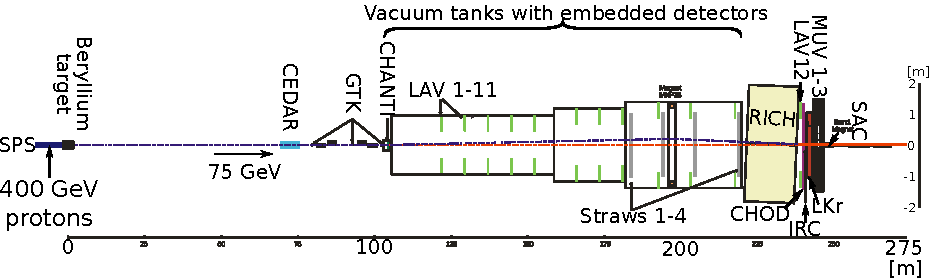
\includegraphics[angle=90,width=1.5in]{na62-overview-en}
\caption{Overview of the NA62 experiment \cite{TDR}.}
\label{fig:na62-overview-en}
\end{figure}

Kaon decay products and beam halo background induce a rate of about 10~MHz in
the sub-detectors. For each event the data of every sub-detector is read out,
leading to a total data rate of about 2.3~TB/s (see Table~\ref{tab:detectors}).

\begin{table}[!t]
% increase table row spacing, adjust to taste
\renewcommand{\arraystretch}{1.3}
\caption{The sub-detectors, their event sizes and the resulting data rates at 10~MHz event rate.}
\label{tab:detectors}
\centering
\begin{tabular}{c|c|c}
		Sub-detector	&	Event size [B] &	Data rate [GBps]\\
		\hline
		CEDAR	&	216		&	2.16	\\
		GTK 	&	2250	&	22.50 	\\
		CHANTI	&	192		&	1.92 	\\
		LAV 	&	160		&	1.60 	\\
		STRAW 	&	768		&	7.68 	\\
		RICH 	&	160		&	1.60 	\\
		CHOD	&	$\ll1000$	&	$\ll10$\\
		MUV 	&	768		&	7.68 \\
		IRC \& SAC 	& 576	& 	5.76 	\\
		\textbf{LKR}		&	\textbf{222~k}	&	\textbf{2220}	\\
		\hline
		\textbf{Sum}	&	\textbf{$\approx$227~kB}	&	\textbf{$\approx$2.3~TB/s}\\
		\end{tabular}
\end{table}


\section{The trigger system}
The maximum data rate with which events can be written to tape is limited by
100~MB/s for the NA62 experiment. To reduce the incoming rate from the detector 
(2.3~TB/s) to this limit, a three level trigger system was developed:
\begin{description}
  \item[L0] FPGA-based readout and trigger (1~ms max. latency)
  \item[L1] Sub-detector level trigger (1~s max. latency)
  \item[L2] Event level trigger (12~s max. latency)
\end{description}

To cope with the high data rates and rigorous real time demands the first level
trigger L0 is implemented in FPGA-based hardware. The higher level
triggers are software architectures running on commodity processors in
large PC farms.

At each positive L0 trigger decision (about 1~MHz) all sub-detectors but the 
Liquid Krypton calorimeter (LKr) are read out by the online PC farm software.
This represents only about 2\% of the data produced by the whole detector and hence induces a data rate of about 5~GB/s (Table~\ref{tab:detectors}). At
L1 the trigger decision is taken based on a partial event reconstruction
and in case of a positive L1 trigger decision ($\sim$100~kHz) the remaining data from the LKr
detector is read out within the time period of a whole beam cycle. As the beam
cycle will be more than two times longer than the proton burst (see section
\ref{sec:dutyCycle}), the LKr data is read out with a data rate of about 7~GBps.
Together with the LKr data the event building takes place and reconstruction
based on the whole detector data is performed (L2). The maximum positive
trigger rate by L2 is limited to about 440~Hz to meet the maximum output data
rate of 100~MB/s.

To reduce the necessary amount of memory within the readout electronics, the
processing time of L0 (L1\footnote{The L1 processing time is limited to reduce
the time until the LKr data is read out which decreases the necessary memory of
the LKr readout electronics.}) is limited to 1~ms (1~s) per event while the
processing time of L2 is only limited by the time between two proton bursts to
reduce the number of necessary PCs.

\begin{figure}[!t]
\centering
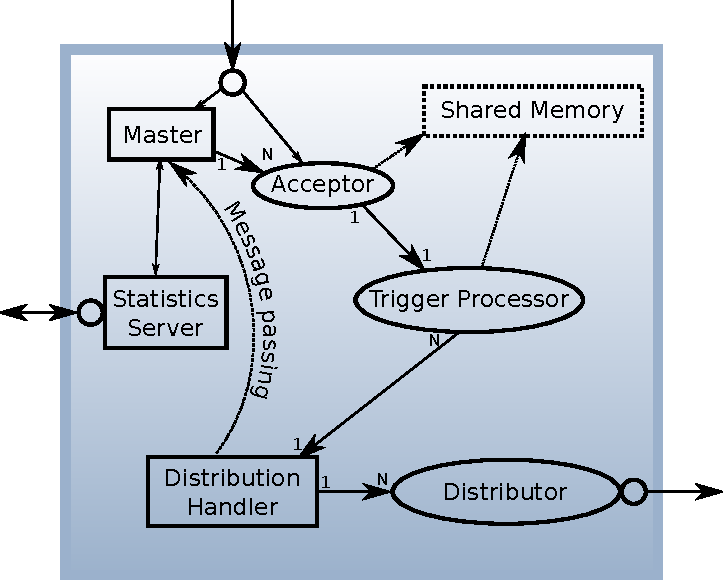
\includegraphics[width=3.5in]{dataflow}
\caption{The logical dataflow from the electronics over the three trigger levels to the tapes.}
\label{fig:dataflow}
\end{figure}



\section{The NA62 online PC farm}
The NA62 PC farm concept physically and logically combines the trigger
levels 1 (L1, sub-detector level) and 2 (L2, event level and event building) into
one single PC farm. This means that each PC can read out and process the data of
every sub-detector and process L1 and L2 algorithms simultaneously. This way
several advantages can be achieved compared to the more common scheme of
separated L1 and L2 farms.


\subsection{L1 event building\label{sec:L1EB}}
Instead of spreading the data of one event over several PCs (sub-component
wise), the digitized raw data of a series of L0-accepted events are sent to one
single farm node, which performs all L1 computations simultaneously as well as
in case of a positive L1 trigger decision the event building and the L2 trigger
decision.

Having the data of all sub-components (except LKr) available at one single PC
a premature event building can be done (L1 event building). This allows to
implement highly efficient trigger algorithms, since each event can be processed
sequentially. As soon as one part of the trigger algorithm declines the event
(e.g. one sub-detector produces a veto signal) the processing can
be stopped for all sub-detectors. In case of distributed event processing this
would not be feasible.

Additionally, due to the L1 event building, no L1 trigger decisions have to be
distributed through the farm. Instead all PCs are running self-sufficiently
making the farm much more scalable.

Even though it is currently planned to implement only L1 algorithms based on the
data of single sub-detectors the L1 event building allows to combine several
sub-components within one algorithm at an early stage of the trigger chain.

\subsection{High scalability and maintainability}
As the combined L1/L2 PC farm is completely homogeneous with respect to the
software, all PCs are optimally used and the system is easily scalable by simple
addition of more computing power. Therefore almost no assumptions on the
performance of the L1 algorithms and PCs need to be made. 

Due to the combination of both trigger levels only one software framework has to
be implemented. Also the installation of the PCs is facilitated as only one
farm has to be maintained.

\subsection{High efficiency\label{sec:dutyCycle}}
Within the NA62 experiment data is only collected during limited
burst periods (T$_\text{b} \approx 5$~s). Between two bursts the out-of-burst
period will last about T$_\text{oob} \approx 12$~s\footnote{These numbers will
vary during the data taking period. The given values are the expected
averages.}.

Due to the negligible latency at L0 (1~ms), the L1 trigger will only read
out data during the burst. As the L1 computation is limited to one second a
separate L1 PC farm would only be processing data for T$_\text{b} +1 \approx
6$~s and stay idle during the remaining time of a burst cycle, namely
T$_\text{oob}-1 \approx 11$~s (see Fig. \ref{fig:bursttime}). This makes the
concept with separate L1/L2 farms very inefficient at fixed-target experiments.

By combining the L1 and L2 PC farms all PCs can be optimally used during the
whole burst cycle (see Fig. \ref{fig:bursttime-merged}). At the NA62 experiment
a separate L1 farm would have only been used about 55\% of the time while only
the L2 farm would have been used efficiently. Estimations show that by joining
the L1 and L2 PC farms to one single homogeneous farm from 10\% up to 25\% of
the whole computing power can be saved here.


\begin{figure}[!t]
\centering
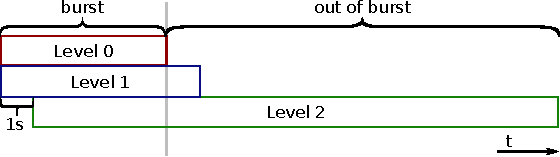
\includegraphics[width=3.5in]{bursttime-eng}
\caption{Processing times of the three different trigger Levels with separate L1/L2 PC farms.}
\label{fig:bursttime}
\end{figure}

\begin{figure}[!t]
\centering
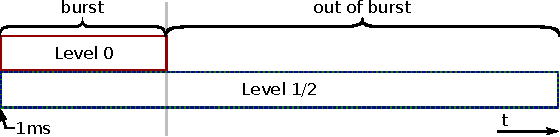
\includegraphics[width=3.5in]{bursttime-l12merged-eng}
\caption{Processing times of the three different trigger Levels with a combined L1/L2 PC farm.}
\label{fig:bursttime-merged}
\end{figure}

\subsection{The topology\label{sec:topology}}
In the final concept the L1/L2 farm PCs are connected via 10~Gb Ethernet through
one 96 port router to the L0 read out electronics. These electronic boards
send bunches of digitized raw data of a series of L0-accepted events to one
single farm node (see section \ref{sec:L1EB}). Each bunch is sent to a
different PC on a Round Robin basis. Events being accepted by L1 and L2 are
sent to the high available merger PC which sorts the events by time and creates
files with all accepted events of one proton burst. These files are sent to a
local buffering disk pool and to a tape library at the CERN computing center
(see figure \ref{fig:topology}).


\begin{figure}[!t]
\centering
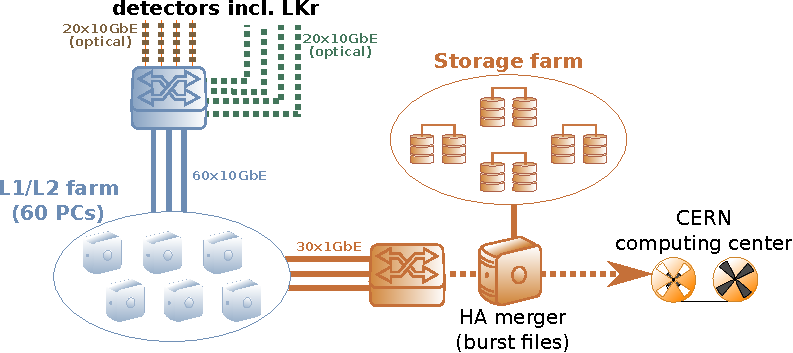
\includegraphics[width=3.5in]{merged-star-eng}
\caption{The final topology of the NA62 PC farm. }
\label{fig:topology}
\end{figure}

\subsection{Drawbacks}
To meet the time limit of the L1 computation the software framework within the
combined PC farm needs to ensure that the L2 processing does not overload the
farm during the burst. This has been implemented via a simple load balancing
algorithm which prioritises the L1 computation. Tests have shown that the
average L1 computation time has become independent of the number of events being
processed by L2 due to this load balancing.

As described in section~\ref{sec:topology} all electronic boards
(except the LKr readout system) send the data of a bunch of events to the same
PC within a very short time. This could potentially overload the main router if
it cannot buffer the short data peak going to one port (PC). At NA62 it is
planned to send bunches of about 10 Events (5~kB each) to one PC. Hence, the buffer size
of the main router must be at the order of 50~kB per port which is small
compared to the typicall buffer sizes of at least the order of 100~kB per Port
at modern Routers. Furthermore, problems related to that unsteady data
transmission can be solved by implementing short delays of different lengths within the
electronic boads.


\section{The software framework}
To receive the raw data from the sub-detectors, to perform the event building,
to initiate the trigger algorithms, and to send the accepted events to the data
storage a C++ based framework was implemented for the NA62 PC farm which is
running on Linux. Tests have shown that using the standard Linux kernel sockets
a relative packet loss of less than $10^{-5}$ at full data rate and high load
using the UDP/IP protocol was not achievable. Therefore the
network communications within the framework are based on a special socket
called \textit{pf\_ring DNA} implemented by the company ntop \cite{pfringDNA}.
Using the \textit{pf\_ring DNA} network driver the data packets are transmitted directly to
the userland memory via direct memory access (DMA). This way the full data rate
of 10~Gb/s can be received without any packet loss and almost no CPU load at
any packet size.

As \textit{pf\_ring DNA} does not yet implement any layer of the UDP/IP protocol
stack, Ethernet, IP, UDP and ARP had to be implemented by the authors. The
resulting framework was tested on a Dell PowerEdge R710 with two Intel
X5675 processors (12 cores and 24 threads total) and 24~GB memory with a clock
frequency of 1333~MHz. The data reception (10~Gb/s), integrity checks, event
building, and the transmission (about 0.1~Gb/s) altogether took less than 25\%
of the whole processing power. Thus, more than 75\% of the processing power of
each PC within the NA62 online PC farm can be used to compute L1 and L2 trigger
algorithms.

\vfill
  

% An example of a floating figure using the graphicx package.
% Note that \label must occur AFTER (or within) \caption.
% For figures, \caption should occur after the \includegraphics.
% Note that IEEEtran v1.7 and later has special internal code that
% is designed to preserve the operation of \label within \caption
% even when the captionsoff option is in effect. However, because
% of issues like this, it may be the safest practice to put all your
% \label just after \caption rather than within \caption{}.
%
% Reminder: the "draftcls" or "draftclsnofoot", not "draft", class
% option should be used if it is desired that the figures are to be
% displayed while in draft mode.
%
%\begin{figure}[!t]
%\centering
%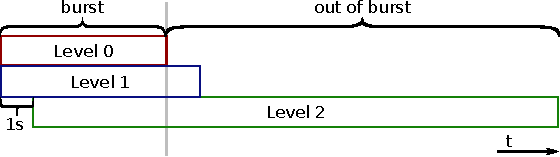
\includegraphics[width=3.5in]{bursttime-eng.pdf}
%% where an .eps filename suffix will be assumed under latex, 
%% and a .pdf suffix will be assumed for pdflatex; or what has been declared
%% via \DeclareGraphicsExtensions.
%\caption{Daily abstract submission rate of the 2012 NSS-MIC. }
%\label{fig_sim}
%\end{figure}


% Note that IEEE typically puts floats only at the top, even when this
% results in a large percentage of a column being occupied by floats.


% An example of a double column floating figure using two subfigures.
% (The subfig.sty package must be loaded for this to work.)
% The subfigure \label commands are set within each subfloat command, the
% \label for the overall figure must come after \caption.
% \hfil must be used as a separator to get equal spacing.
% The subfigure.sty package works much the same way, except \subfigure is
% used instead of \subfloat.
%
%\begin{figure*}[!t]
%\centerline{\subfloat[Case I]\includegraphics[width=2.5in]{subfigcase1}%
%\label{fig_first_case}}
%\hfil
%\subfloat[Case II]{\includegraphics[width=2.5in]{subfigcase2}%
%\label{fig_second_case}}}
%\caption{Simulation results}
%\label{fig_sim}
%\end{figure*}
%
% Note that often IEEE papers with subfigures do not employ subfigure
% captions (using the optional argument to \subfloat), but instead will
% reference/describe all of them (a), (b), etc., within the main caption.


% An example of a floating table. Note that, for IEEE style tables, the 
% \caption command should come BEFORE the table. Table text will default to
% \footnotesize as IEEE normally uses this smaller font for tables.
% The \label must come after \caption as always.
%
%\begin{table}[!t]
%% increase table row spacing, adjust to taste
%\renewcommand{\arraystretch}{1.3}
% if using array.sty, it might be a good idea to tweak the value of
% \extrarowheight as needed to properly center the text within the cells
%\caption{An Example of a Table}
%\label{table_example}
%\centering
%% Some packages, such as MDW tools, offer better commands for making tables
%% than the plain LaTeX2e tabular which is used here.
%\begin{tabular}{|c||c|}
%\hline
%One & Two\\
%\hline
%Three & Four\\
%\hline
%\end{tabular}
%\end{table}


% Note that IEEE does not put floats in the very first column - or typically
% anywhere on the first page for that matter. Also, in-text middle ("here")
% positioning is not used. Most IEEE journals use top floats exclusively.
% Note that, LaTeX2e, unlike IEEE journals, places footnotes above bottom
% floats. This can be corrected via the \fnbelowfloat command of the
% stfloats package.



% if have a single appendix:
%\appendix[Proof of the Zonklar Equations]
% or
%\appendix  % for no appendix heading
% do not use \section anymore after \appendix, only \section*
% is possibly needed

% use appendices with more than one appendix
% then use \section to start each appendix
% you must declare a \section before using any
% \subsection or using \label (\appendices by itself
% starts a section numbered zero.)
%

%\vfill

%\subsection{Submit the Manuscript and Copyright Form}
%After you have obtained the Xplore-compatible PDF file, log on to the NSS-MIC conference web site (http://www.nss-mic.org/2012) using the username and password for your abstract submission.  Go to the ``My Submissions'' link and check that your paper title and author list are consistent with those in your manuscript. Make appropriate changes using the ``Update Abstract'' button if needed. Click on the ``Upload manuscript'' button to transfer your PDF file.  Your PDF file will be checked again for Xplore-compatibility. PDF files that fail the check will not be included in the Conference Record DVD.
%An IEEE Copyright Form should be submitted electronically at the same time your Xplore-compatible manuscript is submitted. Click on the ``Submit Copyright Form'' button on the ``My Abstracts'' link and follow the instructions.  Each manuscript submitted to the Conference Record must be accompanied by a corresponding copyright form. 




%\appendices
%\section{}
%Appendices, if needed, appear before the acknowledgment.

% use section* for acknowledgement
%\section*{Acknowledgment}
%The preferred spelling of the word ``acknowledgment'' in American English is without an ``e'' after the ``g.'' Use the singular heading even if you have many acknowledgments. Avoid the expression, ``One of us (S.B.A.) thanks ...'' Instead, write ``S.B.A. thanks ...'' Put sponsor acknowledgments in the unnumbered footnote on the first page.


% references section

% can use a bibliography generated by BibTeX as a .bbl file
% BibTeX documentation can be easily obtained at:
% http://www.ctan.org/tex-archive/biblio/bibtex/contrib/doc/
% The IEEEtran BibTeX style support page is at:
% http://www.michaelshell.org/tex/ieeetran/bibtex/
%\bibliographystyle{IEEEtran}
% argument is your BibTeX string definitions and bibliography database(s)
%\bibliography{IEEEabrv,../bib/paper}
%
% <OR> manually copy in the resultant .bbl file
% set second argument of \begin to the number of references
% (used to reserve space for the reference number labels box)
\begin{thebibliography}{1}


\bibitem{TDR}
F.~Hahn et al., \emph{Technical Design Document}\hskip 1em plus
  0.5em minus 0.4em\relax NA62 Collaboration, 2010,
  http://na62.web.cern.ch/na62/Documents/TD\_Full\_doc\_v10.pdf
  
\bibitem{Proposal}
G. Anelli et al., \emph{Proposal to measure $K^+\rightarrow
 \pi\nu\bar{\nu}$ rare decay at the CERN SPS}\hskip 1em plus
  0.5em minus 0.4em\relax NA62 Collaboration, CERN-SPSC-2005-013
  
\bibitem{pfringDNA}
http://www.ntop.org/products/pf\_ring/dna/
  

\end{thebibliography}




% that's all folks
\end{document}


